\documentclass[twoside,a4paper,11pt,addpoints]{exam}%answers,



\usepackage{siunitx}
\usepackage{mystyles}
\usepackage[export]{adjustbox}
\usepackage{mathpazo}
\usepackage{booktabs}
\usepackage{framed}
\usepackage{mdframed}
\usepackage[most]{tcolorbox}
\usepackage{listings}
\usepackage{mhchem}
\usepackage{tcolorbox}

\usepackage{subfig}
\usepackage{float}

\lstset
{upquote=true,
columns=flexible,
    basicstyle=\small\tt\hbox{}, 
	basicstyle=\ttfamily,
	language=Python,
    framesep=\fboxsep,
    framerule=\fboxrule,
    xleftmargin=\dimexpr\fboxsep+\fboxrule,
    xrightmargin=\dimexpr\fboxsep+\fboxrule,
	commentstyle=\color{gray},
	frame=single,
	rulecolor=\color{green!5},
	backgroundcolor=\color{gray!5},
	breaklines,
	numbers=left, 
	numbersep=5pt,  
	numberstyle=\scriptsize \ttfamily\color{gray},
	breakindent=1.5em,
	literate={Δ}{{$\mathtt{\Delta}$}}1 {‡}{{$\mathtt{\ddagger}$}}1
  {á}{{\'a}}1 {é}{{\'e}}1 {í}{{\'i}}1 {ó}{{\'o}}1 {ú}{{\'u}}1
  {Á}{{\'A}}1 {É}{{\'E}}1 {Í}{{\'I}}1 {Ó}{{\'O}}1 {Ú}{{\'U}}1
  {à}{{\`a~}}1 {è}{{\`e}}1 {ì}{{\`i}}1 {ò}{{\`o}}1 {ù}{{\`u}}1
  {À}{{\`A~}}1 {È}{{\'E}}1 {Ì}{{\`I}}1 {Ò}{{\`O}}1 {Ù}{{\`U}}1
  {ä}{{\"a}}1 {ë}{{\"e}}1 {ï}{{\"i}}1 {ö}{{\"o}}1 {ü}{{\"u}}1
  {Ä}{{\"A}}1 {Ë}{{\"E}}1 {Ï}{{\"I}}1 {Ö}{{\"O}}1 {Ü}{{\"U}}1
  {â}{{\^a}}1 {ê}{{\^e}}1 {î}{{\^i}}1 {ô}{{\^o}}1 {û}{{\^u}}1
  {Â}{{\^A}}1 {Ê}{{\^E}}1 {Î}{{\^I}}1 {Ô}{{\^O}}1 {Û}{{\^U}}1
  {œ}{{\oe}}1 {Œ}{{\OE}}1 {æ}{{\ae}}1 {Æ}{{\AE}}1 {ß}{{\ss}}1
  {ç}{{\c c}}1 {Ç}{{\c C}}1 {ø}{{\o}}1 {å}{{\r a}}1 {Å}{{\r A}}1
  {€}{{\EUR}}1 {£}{{\pounds}}1 {×}{{$\times$}}1,       
}


\usepackage{adjustbox}
\usepackage{colortbl}
\usepackage{fontawesome}
\usepackage{todonotes}
\usepackage{listings} %codes python
\usepackage{parskip}

\usepackage{subfig}


%Columns Spacing
\newcolumntype{C}[1]{>{\centering\let\newline\\\arraybackslash\hspace{0pt}}m{#1}}
\newcolumntype{M}[1]{>{\centering\arraybackslash}m{#1}}

%Colorbox
\newtcolorbox{mybox}{colback=white!5!white,
colframe=black!75!black,left=7mm}

\newcounter{foo} %Counter questions

\begin{document}



\begin{minipage}{0.33\textwidth}
Noms-Prénoms du binôme
\end{minipage}\begin{minipage}{0.33\textwidth}
$n^\circ 1$ :
\end{minipage}\begin{minipage}{0.33\textwidth}
$n^\circ 2$ :
\end{minipage}
\tito{Synthèse de \ce{TiO2} et conception d'un verre conducteur}

\paragraph*{But} 
Au cours de cette séance de TP, vous réaliserez la formulation d'une électrode à base de dioxyde de titane (\ce{TiO2}) et d'un verre conducteur à base d'oxyde d'indium et d'étain (ITO), deux composants essentiels des cellules solaires à colorant.

%à construire et utiliser des diagrammes binaires. Ceux-ci sont nécessaires à l'interprétation du comportement thermique ou de l'histoire thermique de mélanges solides. De plus, lors de la formation de l'alliage \ce{Pb}-\ce{Sn}, vous utiliserez un four particulier, appelé four tubulaire dont nous discuterons les avantages par rapport au four à moufle.


\paragraph*{Quelques remarques :}
\begin{enumerate}
\item {\color{red} Lors de ces deux séances de TP, il est attendu que vous teniez un cahier de laboratoire : observations, matériel, conditions opératoires doivent être référencées pour permettre le suivi de votre travail.}
\item Toute figure doit comporter des axes, des unités, un titre et des légendes. Le titre doit permettre à l'enseignant de comprendre l'essentiel de la figure sans avoir à lire le texte associé.
\item Toute donnée expérimentale doit être accompagnée des conditions expérimentales et outils associés à la mesure.
\end{enumerate}


\paragraph*{Notations :}
On notera par $X^\star$ une espèce chimique $X$ photoexcitée.

\tableofcontents

\newpage

\`{A} l'ère du dérèglement climatique, il est impératif de trouver une source d'énergie décarbonnée, non polluante et abondante. L'énergie solaire reçue sur Terre est nettement supérieure à la demande énergétique mondiale et peut être utilisée sans produire de pollution, comme le montrent les stratégies photosynthétiques dans le vivant.

En s'inspirant de la photosynthèse, Michael Grätzel a développé les cellules à colorant, une technologie prometteuse parmi les cellules photovoltaïques de troisième génération.

\begin{center}
\begin{minipage}{0.48\textwidth}
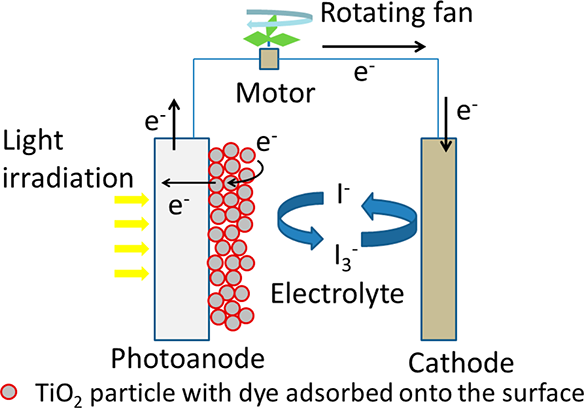
\includegraphics[width=\textwidth]{figures/Fig01}
\end{minipage}\begin{minipage}{0.48\textwidth}
\captionof{figure}{Mécanisme de fonctionnement des cellules solaires à colorant}
\end{minipage}
\end{center}

Les cellules à colorant peuvent être vues comme des photopiles que l'on peut schématiser de la manière suivante : 

\begin{align*}
 ITO (s) | TiO_2(s) | D^+ (ads); D (ads) | I_3^-(aq) ; I^-(aq) | ITO(s)
\end{align*}
où $D$ est une espèce chimique organique, adsorbée à la surface du dioxyde de titane.

Cette pile est constituée de deux demi-piles de troisième espèce, qui mettent en jeux trois couples redox : $D^+(ads) / D(ads)$, $\ce{D^+ (ads)} / \ce{D^\star (ads)}$ et $\ce{I_3^- (aq)} / \ce{I^- (aq)}$.


\section{Questions introductives}

On va chercher à vérifier par un calcul d'ordre de grandeur si l'énergie solaire reçue sur Terre est suffisante pour couvrir la demande énergétique mondiale.

\textbf{Données :}
\begin{itemize}
\item Puissance solaire émise par le soleil : $P_{sol} = \SI{3.8e26}{\watt}$.
\item Rayon moyen de l'orbite terrestre : $d_{T-S} = \SI{1.5e11}{\meter}$.
\item Rayon de la Terre : $R_{T} = \SI{6.4e6}{\meter}$.
\item Consommation énergétique mondiale annuelle : $E_{mondiale} = \SI{5.0e20}{\joule}$.
\item Reflectance moyenne de la Terre : $r = 0.3$.
\end{itemize}

\begin{questions}
\question[2\half] Calculer l'énergie reçue par la Terre en une année. Comparer cette valeur à la consommation énergétique mondiale annuelle.

\begin{mybox}
   \begin{solution}[10cm]
      \textbf{Puissance reçue par la Terre :} [\textbf{1.0}]

      On doit calculer la puissance surfacique reçue par la Terre, en considérant que le Soleil émet de manière isotrope. Faisons un bilan d'énergie :  

      \begin{align*}
         \bar{P}_T = \bar{P}_{sol} - \bar{P}_{ref}
      \end{align*}

      Avec $\bar{P}_T$ la puissance surfacique reçue par la Terre, $\bar{P}_{sol}$ la puissance surfacique émise par le Soleil et $\bar{P}_{ref}$ la puissance surfacique réfléchie par la Terre.

      \begin{align*}
         \bar{P}_T = \frac{P_T}{4 \pi R_T^2} \quad 
         \bar{P}_{sol} = \frac{P_{sol}}{4 \pi d_{T-S}^2} \quad
         \bar{P}_{ref} = r \cdot \bar{P}_{sol} = r \cdot \frac{P_{sol}}{4 \pi d_{T-S}^2}
      \end{align*}

      Donc : 

      \begin{align*}
         P_{T} = P_{sol} \cdot \frac{\pi R_T^2}{4 \pi d_{T-S}^2} \cdot (1-r)
      \end{align*}

      \textbf{Calcul de l'énergie reçue en une année :} [\textbf{1.0}]
      \begin{align*}
         E_T = P_T \cdot \Delta t = P_{sol} \cdot \frac{R_T^2}{4 d_{T-S}^2} \cdot (1-r) \cdot \Delta t
      \end{align*}
      avec $\Delta t = \SI{3.15e7}{\second}$ le temps en une année.
      
      \begin{align*}
         E_T = 3.8 \cdot 10^{26} \cdot \frac{(6.4 \cdot 10^6)^2}{4 \cdot (1.5 \cdot 10^{11})^2} \cdot (1-0.3) \cdot 3.15 \cdot 10^7 = 1.2 \cdot 10^{24} ~ \si{\joule}
      \end{align*}

      \textbf{Comparaison avec la consommation mondiale :} [\textbf{0.5}]
      \begin{align*}
         \frac{E_T}{E_{mondiale}} = \frac{1.2 \cdot 10^{24}}{5.0 \cdot 10^{20}} = 2400
      \end{align*}
      
   \end{solution}
\end{mybox}

   \question[1] Que devrait être l'efficacité minimale des cellules photovoltaïques pour couvrir la consommation énergétique mondiale annuelle ? Quelle est la limite principale de votre calcul ?

   \begin{mybox}
      \begin{solution}[5cm]
         Il faudrait au minimum un rendement de $ \eta = \frac{100}{2400} \approx 4.2 \cdot 10^{-2} ~ \si{\percent} $ pour couvrir la consommation énergétique mondiale annuelle.
         
         La limite de ce calcul est qu'il ne prend pas en compte les pertes liées à la surface effective de captation de l'énergie solaire (océans, nuit, nuages, etc.) et à la surface disponible pour l'installation des cellules photovoltaïques.

         Dans une moindre mesure, il ne prend pas en compte les pertes énergétiques liées au stockage et au transport de l'énergie.
      \end{solution}
   \end{mybox}

\setcounter{foo}{\value{question}}

\end{questions}


\section{Synthèse de \ce{TiO2} par voie micro-onde}

\subsection{Protocole}

%**Matériel nécessaire :**  
%- Solution de TiCl4  
%- Eau distillée  
%- Soude (NaOH) 5 mol.L⁻¹  
%- Acide nitrique (HNO3) 1 mol.L⁻¹  
%- Réacteurs en téflon compatibles avec un four à micro-ondes monomode (type CEM)  
%- Centrifugeuse capable d'atteindre 16 500 tours/min (29 220 g)  
%- Agitateur magnétique  
%- Pipettes graduées et cylindres mésurants  
%- Balance précise  
%- Système de séchage sous vide  

\begin{center}
\begin{minipage}{0.20\textwidth}
\centering
\color{red} \Huge\faWarning
\end{minipage}\begin{minipage}{0.80\textwidth}
\color{red} Manipuler le \ce{TiCl4} avec prudence en raison de sa réactivité avec l'eau et de sa toxicité.
Il faudra prévoir deux DRX : une avant et une après le passage au micro-onde.

Toute les quantités sont indiquées pour la préparation d'une seule suspension. Il faudra diviser les quantités par le nombre de binômes que vous êtes.
\end{minipage}
\end{center}
%\attention{Manipuler le \ce{TiCl4} avec prudence en raison de sa réactivité avec l'eau et de sa toxicité.}

\begin{enumerate}
\item Hydrolyse du \ce{TiCl4} (réalisée par le technicien avant votre arrivée) :
\begin{itemize}
   \item Introduire \SI{14,0}{\milli\liter} de solution de \ce{TiCl4} dans \SI{100}{\milli\liter} d'eau distillée avec précaution.  
   \item Laisser la solution réagir (hydrolyse) à température ambiante pendant une nuit jusqu'à obtention d'une solution limpide.  
\end{itemize}

\item Ajustement du $pH$ :
\begin{itemize}
   \item Ajouter progressivement de la soude à \SI{5}{\mole\per\liter} pour ajuster le $pH$ à $6$ (environ \SI{125}{\milli\liter} nécessaires).  
   \item Agiter la solution pendant \SI{1}{\hour} à l'aide d'un agitateur magnétique.  
   \item Contrôler de nouveau le $pH$ et ajuster si nécessaire. 
\end{itemize}
 

\item Dilution : Compléter la solution avec de l'eau distillée jusqu'à atteindre un volume total de \SI{250}{\milli\liter}, de sorte à obtenir une concentration finale en \ce{Ti^{4+}} de \SI{0.5}{\mole\per\liter}.  

\item Traitement hydrothermal :
\begin{itemize}
   \item Sous agitation, transférer la suspension dans des réacteurs en verre.%téflon.  
   \item Placer les réacteurs dans un four à micro-ondes monomode (CEM).
   \item Chauffer la suspension à \SI{200}{\celsius} en \SI{10}{\minute}, puis maintenir cette température pendant \SI{1}{\hour}.  
   \item La pression interne du réacteur devrait atteindre environ $14$-\SI{15}{\bar}.  
\end{itemize}

\item Récupération du solide  : \`{A} la sortie du réacteur, séparer les suspensions par centrifugation à \SI{6500}{{tour}\per\minute} pendant \SI{20}{\minute}.% 16500 tours/min -> 29220 g 

\item Lavages successifs :
\begin{itemize}
\item Effectuer un premier lavage du précipité à l'eau distillée.  
\item Procéder à un lavage avec de l'acide nitrique (\ce{HNO3}) à \SI{1}{\mole\per\liter}.  
\item Effectuer un dernier lavage à l'eau distillée.  
\end{itemize}

\item Séchage du solide :
\begin{itemize}
\item Placer le solide obtenu dans un système de séchage sous vide à température ambiante.  
\item Laisser sécher pendant une nuit. 
\end{itemize} 
\end{enumerate}

%- Porter des équipements de protection individuelle (gants, lunettes, blouse de laboratoire).  
%- Effectuer les manipulations sous hotte aspirante lorsque nécessaire.  

Ce protocole permet d'obtenir un solide à base de titane par méthode hydrothermale.

\subsection{Questions sur la synthèse de \ce{TiO2}}

\begin{questions}
\setcounter{question}{\thefoo}

\question[1] Écrire l'équation d'hydrolyse du \ce{TiCl4} en milieu aqueux en supposant que l'hydrolyse est totale.

\begin{mybox}
\begin{solution}[5cm]
\begin{align*}
\ce{TiCl4 (aq)+ 4 HO^-(aq) -> Ti(OH)4 (aq) + 4 Cl^- (aq)}
\end{align*}

Sous la forme d'un aquacomplexe, on pourrait écrire : 
\begin{align*}
   \ce{Ti(OH)_4 (H2O)_2}
\end{align*}

\end{solution}
\end{mybox}


\question[2] Justifier que le technicien ait laissé la solution s'hydrolyser pendant toute la nuit.

\begin{mybox}
\begin{solution}[5cm]

\ce{Cl-} est un ligand plus dur \ce{H2O}. Le \ce{Ti} étant à haut degré d'oxydation, il est probablement assez dur, rendant le complexe relativement \textbf{inerte} en présence d'eau.  L'hydrolyse du complexe de \ce{Ti(IV)} est probablement très lente.
\end{solution}
\end{mybox}

\question On va commencer par déterminer les concentrations de travail.

\begin{parts}
\part[1] Calculer la concentration en titane ($IV$) préparée par le technicien.

\begin{mybox}
\begin{solution}[8cm]

\begin{align*}
C_{\ce{Ti(IV)}} = \frac{\rho V_0}{M(\ce{TiCl4}) (V_0+\Delta V)}
\end{align*}

avec $\rho$ la masse volumique de \ce{TiCl4}, $V_0$ le volume prélevé de la solution de \ce{TiCl4}, $M$ la masse molaire de \ce{TiCl4}, $\Delta V$ le volume d'eau ajouté.

\textbf{NB :} Il y a une erreur conceptuelle dans ce calcul, puisque qu'il n'y a pas de raison que le volume du mélange \ce{TiCl4-H2O} fasse \SI{114}{\milli\liter}. Il est fort probable qu'il y a ait contraction du volume lors du mélange, donc que $V_{réel} <  V_0 + \Delta V$.

\textbf{AN :}
\begin{align*}
C_{\ce{Ti(IV)}} = \frac{1.726 \times 14}{189.7 \times 0.114} = 1.12 ~ \si{\mole\per\liter}
\end{align*}


\end{solution}
\end{mybox}

\part[1] Calculer la concentration en titane ($IV$) de votre solution définitive.
\begin{mybox}
\begin{solution}[5cm]
On regarde la relation de dilution :
\begin{align*}
C'_{\ce{Ti(IV)}} = \frac{C_{\ce{Ti(IV)}} V_p}{V'}
\end{align*}

avec $V_p$ le volume prélevé et $V'$ le volume après dilution.

Sinon on peut estimer à partir de la quantité d'hydroxyde ajouté :
\begin{align*}
C'_{Ti(IV)} = \frac{n_{\ce{HO-}}}{4 V'} = \frac{C_{NaOH} V_E}{4 V'}
\end{align*}

avec $V_E$ le volume équivalent de solution de \ce{NaOH} ajoutée et $C_{\ce{NaOH}}$ la concentration en \ce{NaOH} dans la solution préparée.
\end{solution}
\end{mybox}
\end{parts}

\setcounter{foo}{\value{question}}
\end{questions}

\subsection{Caractérisation de la phase par DRX}

\begin{questions}

\setcounter{question}{\thefoo}

\question[1] Commenter l'utilité du micro-ondes en vous appuyant sur les données DRX.

\begin{mybox}
\begin{solution}[5cm]

\textbf{Utilité du micro-ondes :} [\textbf{1.0}]
\begin{itemize}
\item Chauffage uniforme ;
\item Diminution des latences par rapport à un chauffage traditionnel ;
\item Accéleration de la cinétique de formation des matériaux nanoparticulaires.
\end{itemize}

\textbf{Bilan :} [\textbf{1.0}] Meilleur contrôle de la nucléation et de la croissance des nanoparticules, limitant les effets indésirables comme l'agrégation (murissement) nanoparticulaires.

\end{solution}
\end{mybox}

\question[5] Caractériser la (ou les) phase(s) formée(s). Est-on plutôt sur un matériau bulk ou sur des nanoparticules ?

\begin{mybox}
\begin{solution}[5cm]

\textbf{Comparaison $d_{hkl}$ aux tables :} [\textbf{2.0}]

\textbf{Commentaire nature du matériau :} [\textbf{1.0}] Largeur des pics caractéristique de nanoparticules.

\textbf{Détermination des paramètres $a$ et $c$ :} [\textbf{2.0}]

\begin{align*}
d_{hkl} = \frac{1}{\sqrt{\frac{h^2 + k^2}{a^2} + \left(\frac{l}{c}\right)^2 }}
\end{align*}

\end{solution}
\end{mybox}

Il est montré que les nanoparticules d'anatase et de rutile croissent selon des directions privilégiées en fonction des conditions hydrothermales utilisées. Pour simplifier, nous considérerons que les nanoparticules croissent selon la direction $\vec{c}$.

\question

\begin{parts}
\part[4]Proposer des plans réticulaires qui permettrait de comparer la croissance des deux phases le long de la direction privilégiée. Pour cela, on pourra s'aider de représentations schématiques des familles de plans réticulaires.

\begin{mybox}
\begin{solution}[8cm]
\textbf{Plans réticulaires :} [\textbf{1.0}]
\begin{itemize}
\item Rutile : $(002)$
\item Anatase : $(004)$
\end{itemize}
\end{solution}
\end{mybox}

\part[2] En vous aidant des données DRX, vérifier qualitativement l'hypothèse de croissance préférentielle le long de la direction $\vec{c}$.
\begin{mybox}
\begin{solution}[5cm]
\textbf{Démarche} [\textbf{1.0}]
Comparer la largeur des pics caractéristiques des plans $(002)$ et $(004)$ aux autres pics.\\
\textbf{Résultat} [\textbf{1.0}]
Les pics $(002)$ et $(004)$ sont plus larges que les autres pics, ce qui confirme l'hypothèse de croissance préférentielle le long de la direction $\vec{c}$.
\end{solution}
\end{mybox}

\end{parts}

%Il est possible à partir de la DRX de caractériser la forme et la taille typique de la nanoparticules. En particulier, dans notre système, la morphologie des nanoparticules est connue, ainsi que l'orientation des plans réticulaires :
%\begin{center}
%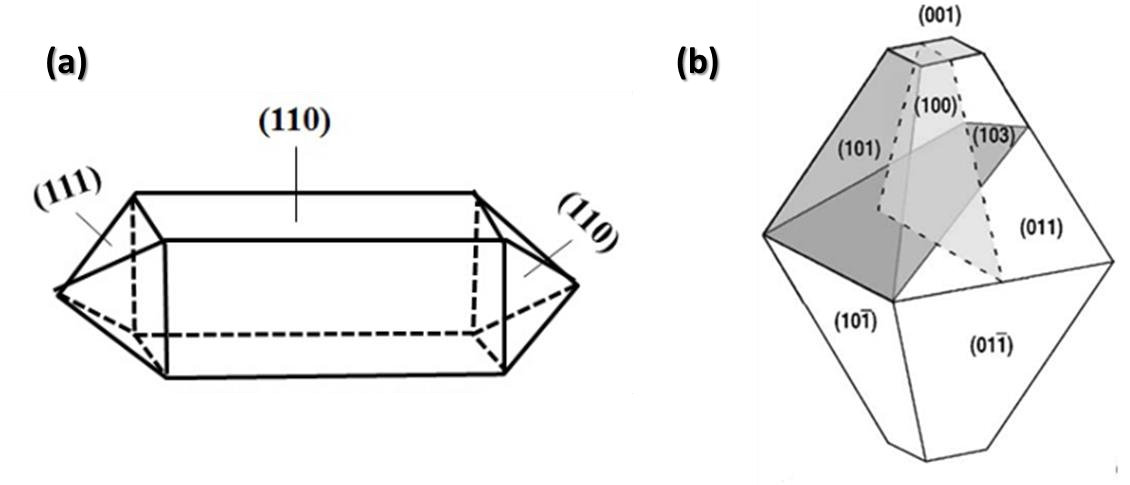
\includegraphics[width=0.8\textwidth]{figures/Fig04a}
%\captionof{figure}{Morphologie type des nanoparticules de \textbf{(a)} rutile et \textbf{(b)} d'anatase}
%\end{center}

\question[6] \`{A} partir de vos acquisitions DRX et de tout modèle qui vous semblera pertinent, caractériser, si possible, l'anisotropie des nanoparticules formées.

\begin{mybox}
\begin{solution}[8cm]

\textbf{Démarche} [\textbf{1.0}] On peut utiliser la formule de Scherrer pour estimer la taille des nanoparticules à partir de la formule de Laue-Scherrer : 
\begin{align*}
L_{hkl} = \frac{0.89 \lambda}{\sqrt{H_{hkl}^2 - s^2} \cos \theta}
\end{align*}

avec $L_{hkl}$ la largeur du pic dans la direction $[hkl]$, $H_{hkl}$ la largeur à mi-hauteur de l'interférence associée à la famille $(hkl)$, en $rad$, et $s$ l'élargissement "naturel" des pics dû à l'instrumentation et $\theta$ l'angle de diffraction (c-a-d la moitié de celui du diffractogramme).

\textbf{Simplification} [\textbf{1.0}] On se place dans un cadre simplificateur où $H_{hkl} \gg s$, ce qui permet d'estimer au premier ordre la dimension des particules dans les différentes directions : 
\begin{align*}
L_{hkl} \approx \frac{0.89 \lambda}{ H_{hkl} \cos \theta}
\end{align*}

\textbf{Estimation} [\textbf{2.0}] $\lambda = 0.1542$

\begin{center}
\begin{tabular}{cccccc}
\toprule
Plans & $(101)$ & $(004)$ & $(200)$ & $(105)$ & $(204)$ \\
\midrule
$H$ [\si{\centi\meter}] & $0.5$ & $0.5$ & $0.6$ & $0.8$ & $0.5$ \\
$H$ [\si{{rad}}] & $2.42 \cdot 10^{-2}$ & $2.42 \cdot 10^{-2}$ & $2.91 \cdot 10^{-2}$ & $3.88 \cdot 10^{-2}$ & $2.42 \cdot 10^{-2}$ \\
$L_{hkl}$ [\si{\nano\meter}] & $5.88$ & $6.07$ & $5.22$ & $4.02$ & $6.72$ \\
\bottomrule
\end{tabular}
\end{center}

~\

\textbf{\color{red} Mise en relation avec la forme des nanoparticules} IMPOSSIBLE -> soucis sur les schémas précédents.

Particules de quelques nanomètres -> grande surface spécifique ? [\textbf{1.0}] ?

\textbf{Autres méthodes plus avancées} [\textbf{1.0}] Méthode de Scherrer, affinement de Rietveld.

\end{solution}
\end{mybox}

\setcounter{foo}{\value{question}}

\end{questions}

\newpage 

\section{Tables DRX}

\begin{center}
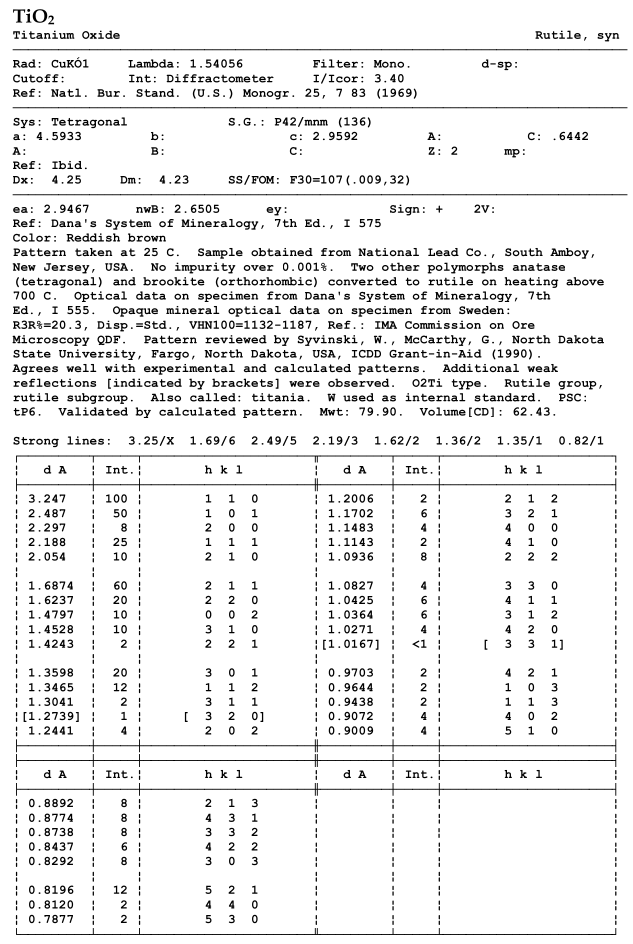
\includegraphics[width=\textwidth]{figures/Ann01}
\end{center}

\begin{center}
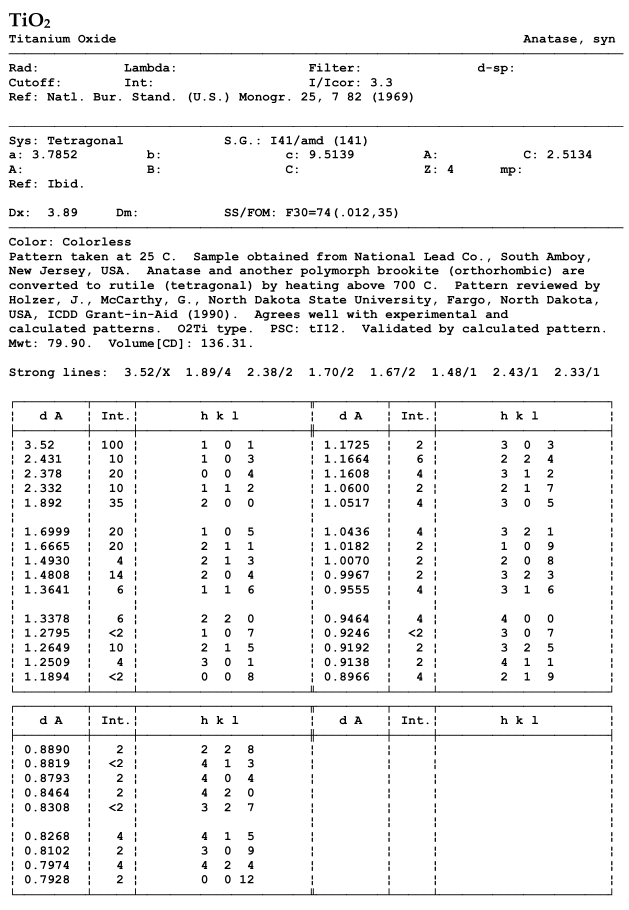
\includegraphics[width=\textwidth]{figures/Ann02}
\end{center}

\newpage

\begin{minipage}{0.33\textwidth}
Nom-Prénom de l'étudiant
\end{minipage}\begin{minipage}{0.33\textwidth}
$n^\circ 1$ :
\end{minipage}

\section{Approfondissement}

   \subsection{Principe de la cellule de Grätzel}
Nous allons chercher à utiliser les données et documents suivants afin de comprendre les propriétés fonctionnement de la cellule de Grätzel 


\begin{figure}[H]
\begin{center}
\begin{tabular}{cc}
\subfloat[\label{fig:TP1-02a}]{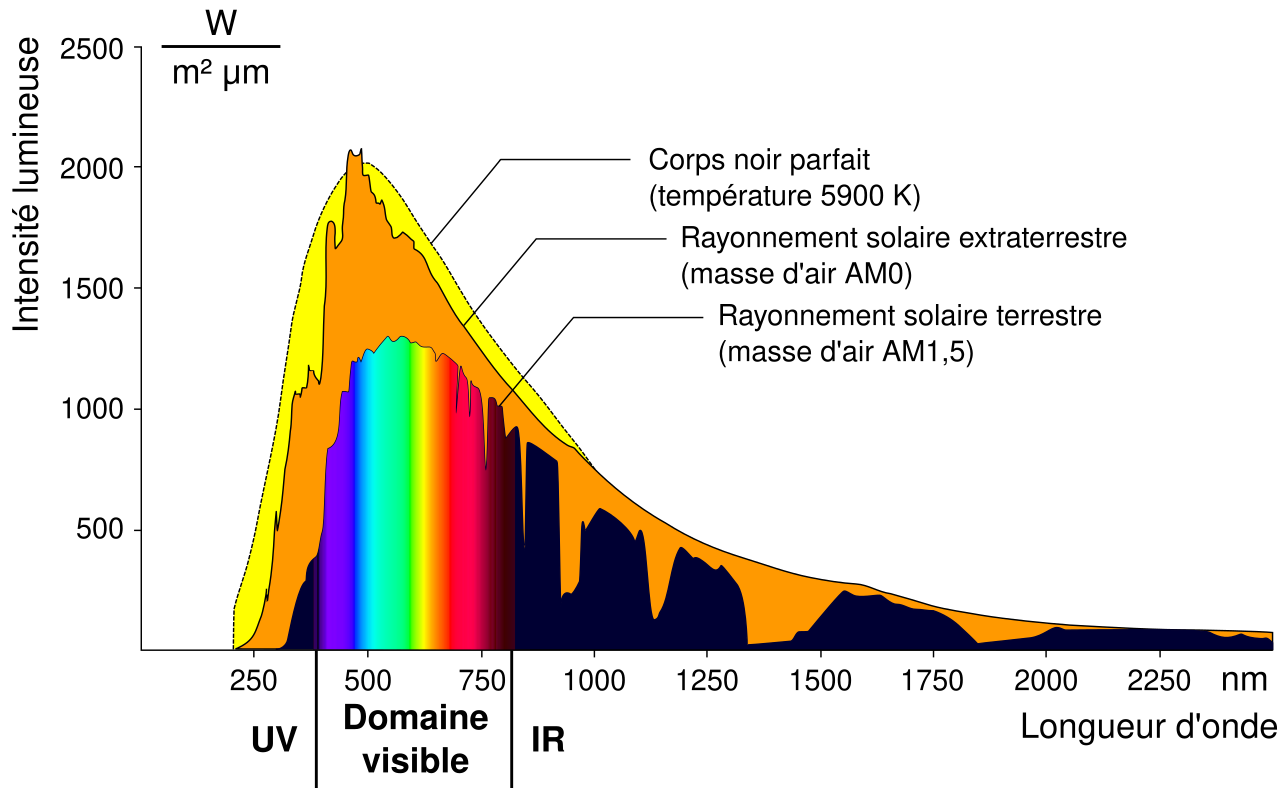
\includegraphics[width=7cm]{figures/Fig02a}} & \subfloat[\label{fig:TP1-02b}]{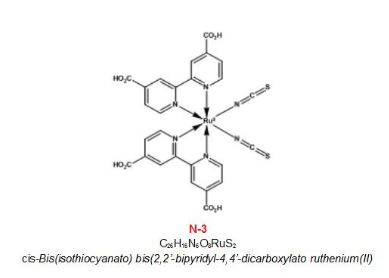
\includegraphics[width=7cm]{figures/Fig02b}} \\
\subfloat[\label{fig:TP1-02c}]{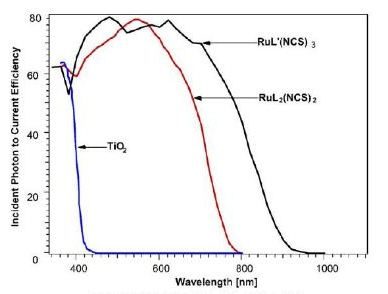
\includegraphics[width=7cm]{figures/Fig02c}} & \subfloat[\label{fig:TP1-02d}]{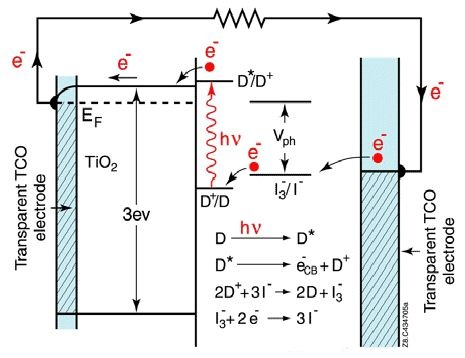
\includegraphics[width=7cm]{figures/Fig02d}} %\\
%\subfloat[\label{fig:TP1-02e}]{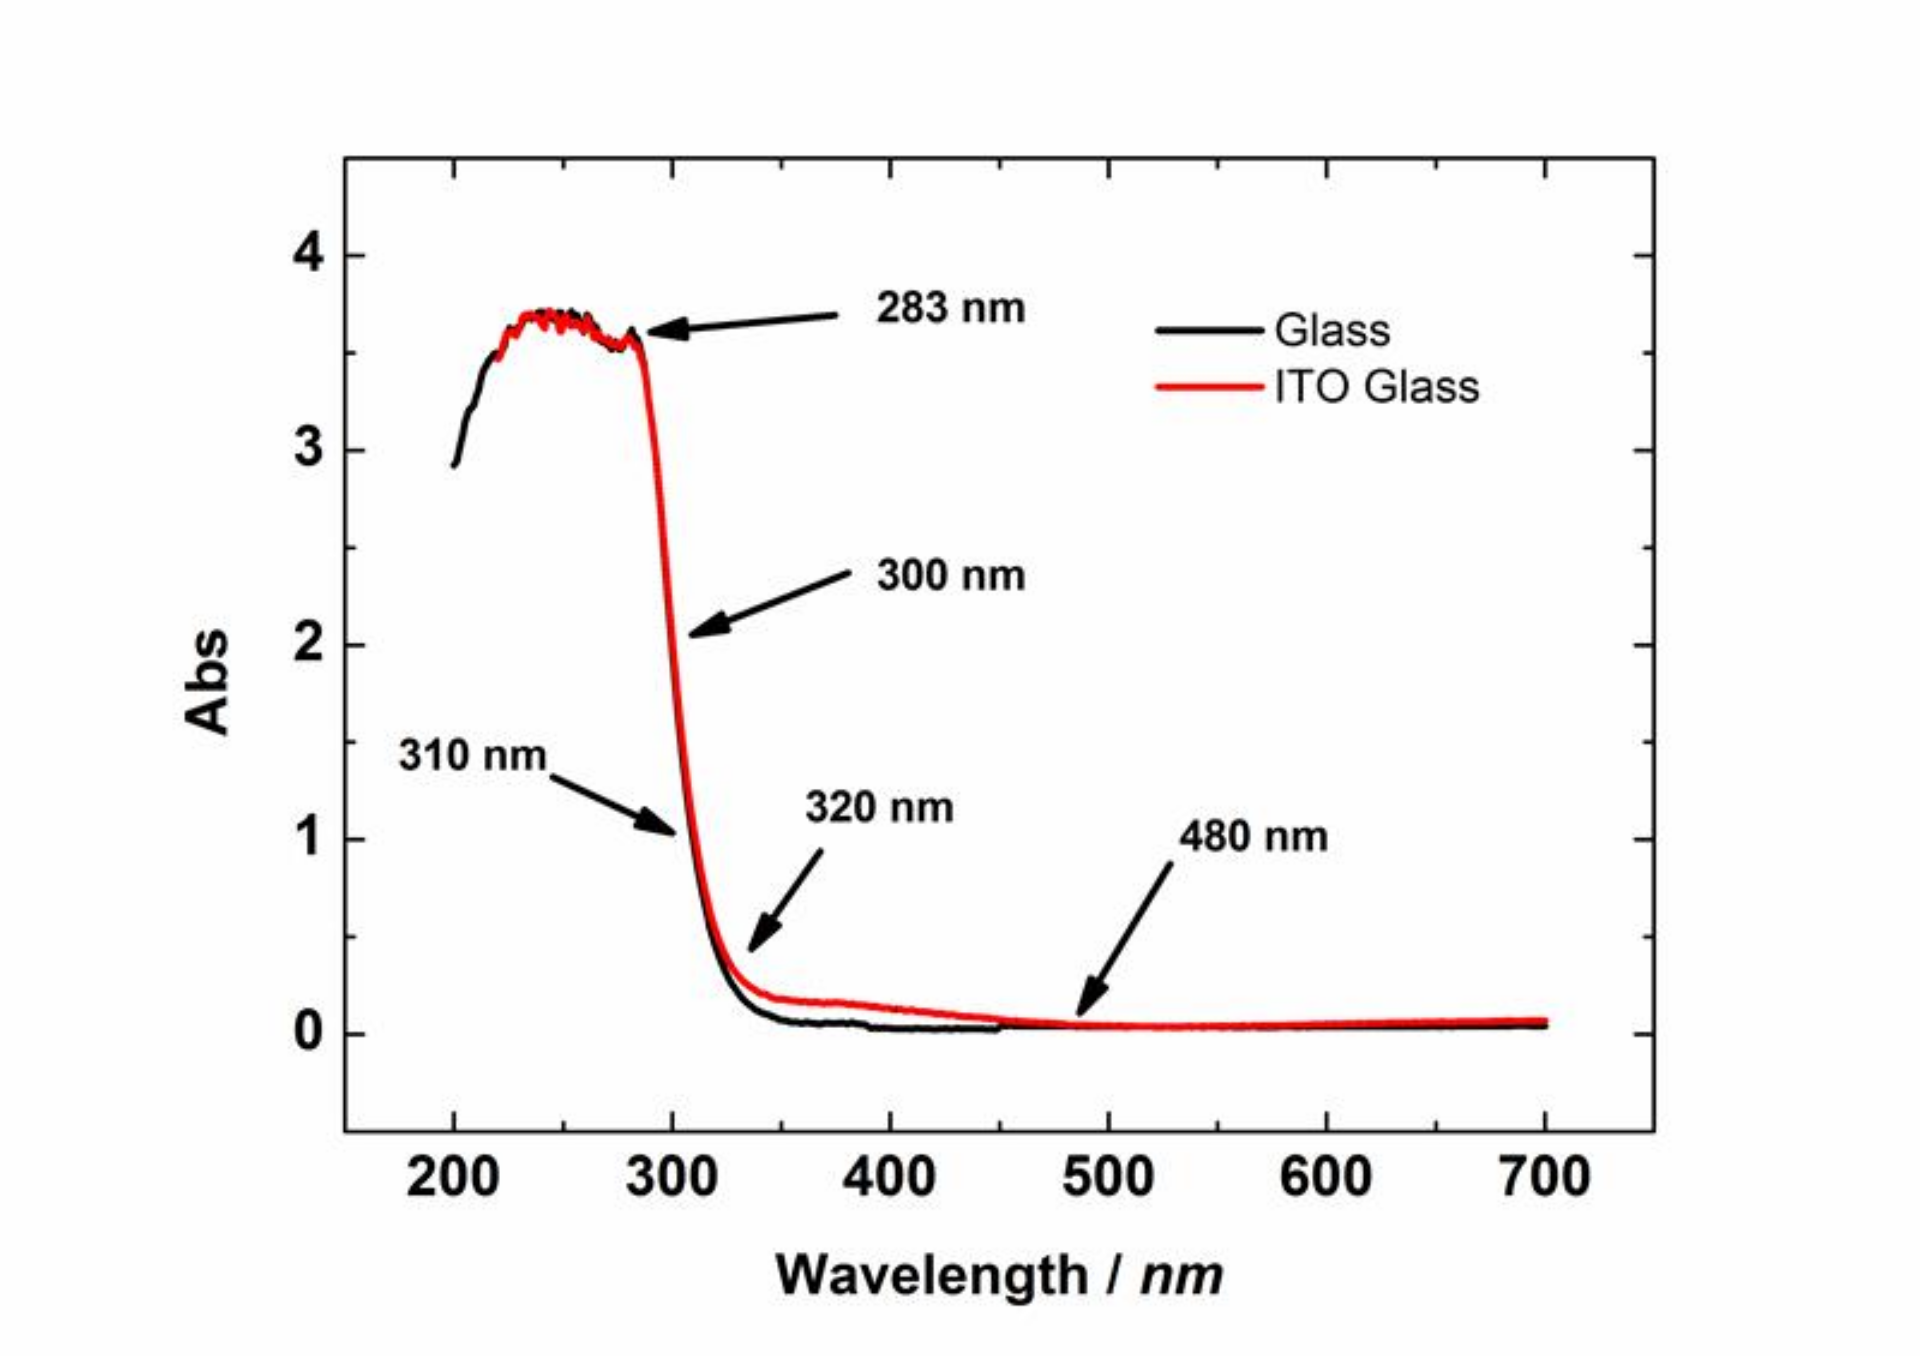
\includegraphics[width=7cm]{figures/Fig02e}} & \\
\end{tabular}
\end{center}
\caption{\ref{fig:TP1-02a} Spectre du rayonnement solaire avant et après traversée de l'atmosphère ; \ref{fig:TP1-02b} Colorant, aussi appelé chromophore $N_3$, servant de référence dans les cellules de Grätzel ; \ref{fig:TP1-02c} Spectre de génération du photocourant en fonction de la longueur d'onde de l'onde incidente à puissance constante ; \ref{fig:TP1-02d} Représentation schématique du processus.}% ; \ref{fig:TP1-02e} Spectre d'absorption normalisé du verre avec et sans dépôt d'ITO.}
\end{figure}

\begin{questions}
\setcounter{question}{\thefoo}

\question[1\half] Identifier l'anode, la cathode et les pôles de cette pile.

\begin{mybox}
\begin{solution}[5cm]

\begin{center}
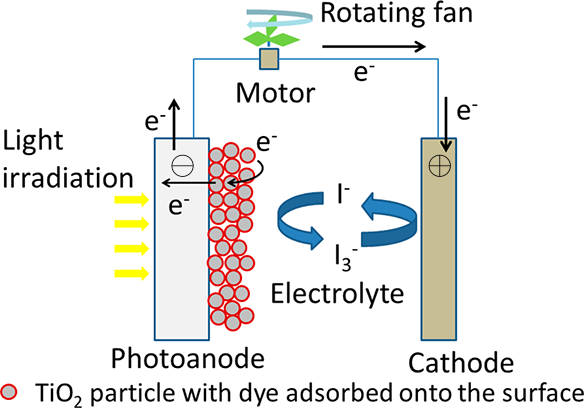
\includegraphics[width=0.4\textwidth]{figures/Corr01}
\end{center}

\textbf{Barême :} $0.5 \times 3$

\end{solution}
\end{mybox}

\question[1\half] Pourquoi ne se contente-t-on pas d'un verre conducteur, d'un colorant et d'une contre-électrode dans un tel dispositif ?

\begin{mybox}
\begin{solution}[5cm]

Dans la cellule, il y a deux éléments en plus des trois cités ci-dessus : 
\begin{enumerate}
\item le pigment, déposé à la surface du verre conducteur, qui permet la conversion d'énergie sert de médiateur rédox entre le colorant adsorbé à sa surface et l'électrode (collecteur de courant) ; \textbf{[0.5]}
\item l'électrolyte qui permet la migration des ions entre demi-piles, tout en servant d'espèce rédox à la cathode (réduction du diode en iodure). \textbf{[0.5]}
\end{enumerate}

En l'absence d'un de ces éléments, le "circuit" est ouvert et on ne peut générer de photocourant. \textbf{[0.5]}

\textbf{NB :} la surface spécifique de \ce{TiO2} nanoparticulaire peut être discutée même si aucun des documents n'invite à le faire.

\end{solution}
\end{mybox}

\question[3] Sur un axe de potentiel, représenter les potentiels rédox standard des couples rédox mis en jeu dans la photopile. Quel est l'intérêt de la lumière du point de vue rédox ? \'{E}crire l'équation rédox associée.

\begin{mybox}
\begin{solution}[5cm]
\textbf{Allure de l'axe de potentiel : [1.5]}  En s'appuyant sur la Fig. \ref{fig:TP1-02d}, où l'évolution en énergie des états électroniques est représentée dans le sens inverse du potentiel rédox.

\begin{center}	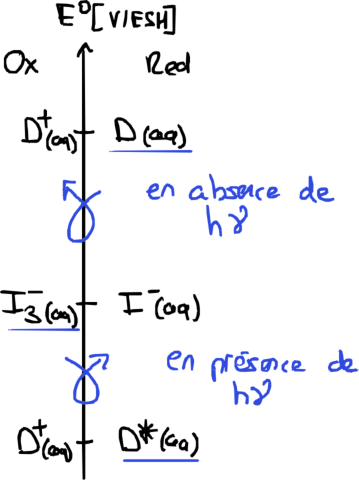
\includegraphics[width=0.25\textwidth]{figures/Corr02}
\end{center}

\textbf{Interprétation de l'effet de la lumière : [1.0]} En absorbant un photon, le colorant passe d'un état électronique fondamental à un état électronique excité. Ceci se manifeste du point de vu rédox par une diminution du potentiel rédox standard du couple, et par conséquent, une plus grande facilitée à s'oxyder.

\textbf{Equation de réaction thermodynamiquement favorisée : [0.5]}

\begin{align*}
\ce{I3^- (aq) + 2  D^\star (aq) = 2 D+(aq) + 3 I-(aq)}
\end{align*}

\end{solution}
\end{mybox}

\question[1\half] Grätzel a développé toute une famille de colorants autour des complexes de ruthénium, dont la structure du $N-3$ est formulée à la Fig. \ref{fig:TP1-02b}. Quel est l'apport du colorant ?

\begin{mybox}
\begin{solution}[5cm]

La Fig. \ref{fig:TP1-02c} présente l'efficacité de la conversion des photons en courant induit par l'effet photovoltaïque à différente longueurs d'onde, pour différents colorants. En l'absence de colorant (témoin), on a présence uniquement de \ce{TiO2} et donc aucun courant pour les induits par les photons visibles. Ceci est à mettre en relation avec le caractère isolant de \ce{TiO2} ($E_g \approx 3 \si{\electronvolt}$ d'après la Fig. \ref{fig:TP1-02d}, fonction du polymorphe).

D'un autre côté, la colorants proposé par l'équipe de Graëtzel présence des ligands fortement conjugué garantissant des transitions dans le visible. Ces colorants, probablement dû à leur centre métallique, présentent aussi la capacité de transférer des électrons vers les électrodes. Par conséquent, et au vu des du spectre de rayonnement solaire, cf. Fig. \ref{fig:TP1-02a}, on compte assez facilement que la majorité des photons étant dans le visible, il est nécessaire d'avoir un colorant absorbant dans le visible, avec des propriétés rédox, pour augmenter le rendement de conversion de la lumière solaire en courant.
\end{solution}
\end{mybox}

%De manière contre-intuitive, les semi-conducteurs à petit gap d'énergie présentent des rendements plus faibles que ceux à grand band gap, justifiant en partie l'utilisation de \ce{TiO2}.
%
%\question[1] {\color{red} Identifier une origine physique possible à cette observation.}
%
%\begin{mybox}
%\begin{solution}[5cm]
%
%Un photon fournit une énergie de minimale valant $Eg$. Or, on sait que le travail récupérable du point de vu électrique est fixé par la position du niveau de Fermi.
%
%Ainsi, si les électrons avec une énergie nettement supérieure à l'énergie de gap, ceci conduira à de nombreuses pertes par d'énergie thermique. De plus, le processus de recombinaison est d'autant plus important que le gap est petit.
%
%\end{solution}
%\end{mybox}
%
%\question[2] {\color{red} Sur la base des données ci-dessus, proposer un cahier des charges des propriétés que doit satisfaire l'ITO dans une cellule photovoltaïque.}
%
%\begin{mybox}
%\begin{solution}[5cm]
%On peut lister un ensemble de contraintes techniques :
%\begin{enumerate}
%\item Transparence élevée dans le visible ;
%\item Conductivité électriques élevée ;
%\item Stabilité photochimique, chimique et thermique ;
%\item Adhérence au verre.
%\end{enumerate}
%
%\end{solution}
%\end{mybox}

\setcounter{foo}{\value{question}}
\end{questions}


%http://physique.unice.fr/sem6/2011-2012/PagesWeb/PT/Cellule/colorant.html



\subsection{Analyse du protocole}

%\begin{center}
%\begin{minipage}{0.58\textwidth}
%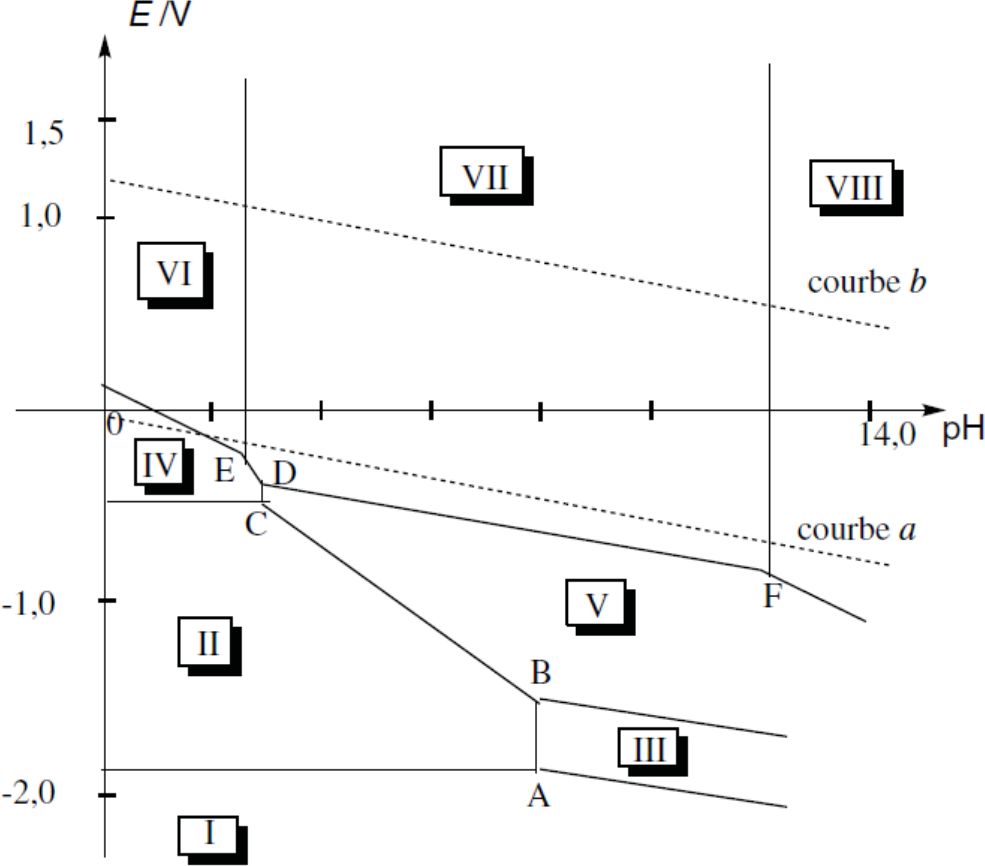
\includegraphics[width=\textwidth]{figures/Fig03}
%\end{minipage}\begin{minipage}{0.38\textwidth}
%\captionof{figure}{Diagramme $E-pH$ du titane à \SI{298}{\kelvin} et à une concentration de tracée {\color{red} $c_{tr}$}}
%\end{minipage}
%\end{center}
%\begin{questions}


%Les espèces du titane suivantes en solution aqueuses sont identifiées et ont été utilisées pour modéliser le diagramme $E-pH$ : \ce{Ti^{2+}(aq)}, \ce{Ti^{3+}(aq)}, \ce{TiO^{2+}}(aq)}, \ce{HTiO_3^{-}(aq)}, \ce{Ti(s)}, \ce{Ti(OH)2(s)}, \ce{Ti(OH)3(s)} et \ce{TiO(OH)2(s)}.

%\question Affecter les domaines à chacune des espèces ci-dessus en justifiant proprement vos choix.

%\question Quelles sont les espèces stables dans l'eau désaérée ? Et dans l'eau aérée ?

%Il a été observé expérimentalement qu'au moment de l'hydrolyse de \ce{TiCl4(l)}, la solution se trouble.

%\question Identifier l'espèce formée au début de l'hydrolyse de \ce{TiCl4(l)}.

%\question Que se passe-t-il lorsque la solution devient limpide ? \'{E}crire le processus associé à cette réaction.

Les processus de synthèse de \ce{TiO2} est réalisé par une succession de condensations nécessitant le départ d'un précurseur monomérique de formule brut : 

\begin{align*}
\ce{[Ti (OH)_h (H2O)_{6-h}]^{4-h}}
\end{align*}

avec $h$ la st{\oe}chiométrie en ions hydroxyde dans le complexe, aussi appelé taux d'hydrolyse.



Le taux d'hydrolyse du titane hydraté à température ambiante a été "étalonné" en fonction du $pH$ de la solution 

\begin{align}
h = \frac{1.0584 + 0.3181 pH}{0.6794 + 0.01776 pH}
\label{eq:h_Tamb}
\end{align}

\begin{questions}
\setcounter{question}{\thefoo}

\question Nous allons chercher à caractériser les complexes de titane précurseurs éventuellement formés.

\begin{parts}
\part[3] Tracer l'évolution du taux d'hydrolyse. Commenter cette évolution et annoter si elle fait sens chimiquement. 

\begin{mybox}
\begin{solution}[5cm]

\begin{center}
\begin{minipage}{0.68\textwidth}
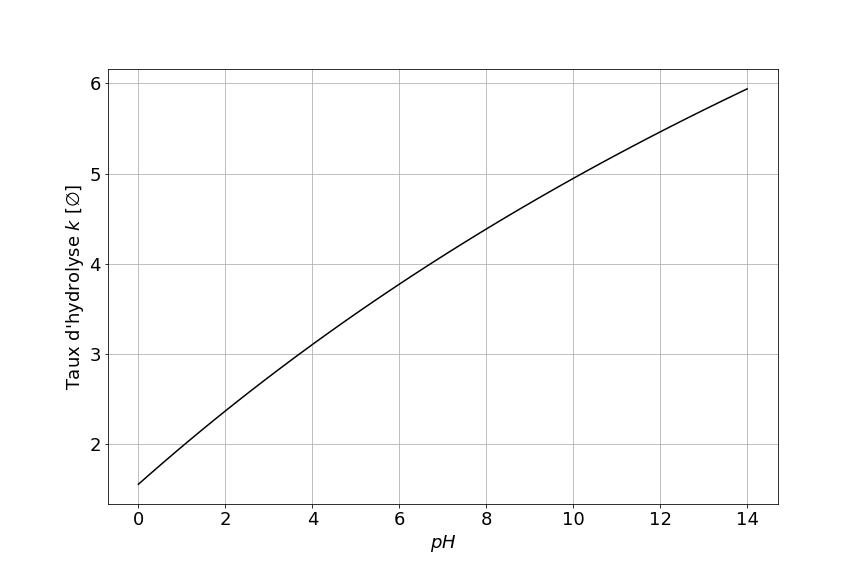
\includegraphics[width=\textwidth]{figures/Corr03}
\end{minipage}\begin{minipage}{0.28\textwidth}
\captionof{figure}{Evolution du taux d'hydrolyse en fonction du $pH$}
\end{minipage}
\end{center}


On remarque que le taux d'hydrolyse évolue de manière monotone, non linéaire et croissant avec le pH. Ceci fait sens, puisque lorsqu'on hydrolyse le composé, on s'attend à une diminution du nombre de ligand aqua et une augmentation du nombre de ligand hydroxo par déprotonations successives. 


\end{solution}
\end{mybox}

\part[3\half] En déduire les $pK_a$ du titane aqueux à \SI{25}{\celsius} et représenter le diagramme de prédominance du titane à cette température.

\begin{mybox}
\begin{solution}[5cm]
\textbf{Méthodologie} [\textbf{1.0}] 
Les équations de réaction successives associées aux aquacomplexes de \ce{Ti(IV)} peuvent s'écrire : 
\begin{align*}
\ce{[Ti (OH)_h (H2O)_{6-h}]^{4-h} (aq) = [Ti (OH)_{h+1} (H2O)_{6-(h+1)}]^{4-(h+1)} (aq) + H^+(aq) } \quad K_{A, h+1}
\end{align*}

avec $h$ entier ici !!!!

On sait que dans un mélange de Henderson, constitué de l'acide et de sa base conjuguée, le pH est donné par : 
\begin{align*}
pH = pK_{a, h+1} + \log \frac{\left[ \ce{[Ti (OH)_h (H2O)_{6-h}]^{4-h} (aq)} \right]}{\left[ \ce{[Ti (OH)_{h+1} (H2O)_{6-(h+1)}]^{4-(h+1)} (aq)} \right]}
\end{align*}

Or, pour que $pH = pK_{A,h}$, il faut que $\left[ \ce{[Ti (OH)_h (H2O)_{6-h}]^{4-h} (aq)} \right] = \left[ \ce{[Ti (OH)_{h+1} (H2O)_{6-(h+1)}]^{4-(h+1)} (aq)} \right]$, ce qui se traduit en apparence par un taux d'hydrolyse moyen valant $h + \frac{1}{2}$.

\textbf{Détermination des pKa} [\textbf{2.0}] 
On inverse l'Eq. \ref{eq:h_Tamb}

\begin{align*}
pH = \frac{0.6794 \cdot h - 1.0584}{0.3181 - 0.01776 \cdot h}
\end{align*}


\begin{center}
\begin{minipage}{0.78\textwidth}
\begin{tabular}{ccc}
\toprule
Couple & $h$ & $pK_A$ \\
\midrule
\ce{[Ti(OH)0(H2O)_6]^{4+} (aq) / \ce{[Ti(OH)1(H2O)_5]^{3+} (aq)}} & $0.5$ & $-2.32$ \\
\ce{[Ti(OH)1(H2O)_5]^{4+} (aq) / \ce{[Ti(OH)2(H2O)_4]^{3+} (aq)}} & $1.5$ & $-0.13$ \\
\ce{[Ti(OH)2(H2O)_4]^{4+} (aq) / \ce{[Ti(OH)3(H2O)_3]^{3+} (aq)}} & $2.5$ & $2.34$ \\
\ce{[Ti(OH)3(H2O)_3]^{4+} (aq) / \ce{[Ti(OH)4(H2O)_2]^{3+} (aq)}} & $3.5$ & $5.16$ \\
\ce{[Ti(OH)4(H2O)_2]^{4+} (aq) / \ce{[Ti(OH)5(H2O)_1]^{3+} (aq)}} & $4.5$ & $8.39$ \\
\ce{[Ti(OH)5(H2O)_1]^{4+} (aq) / \ce{[Ti(OH)6(H2O)_0]^{3+} (aq)}} & $5.5$ & $12.15$\\
\bottomrule
\end{tabular}
\end{minipage}\begin{minipage}{0.18\textwidth}
\captionof{table}{pKa déterminés à partir de l'inversion de l'Eq. \ref{eq:h_Tamb}}
\end{minipage}


\textbf{Commentaire :} [\textbf{0.5}]
Dans l'eau (sous couvert qu'il soit bien le composé largement majoritaire), on peut donc trouver 4 complexes en fonction du pH avec un taux d'hydrolyse $h \in [2,6])$.

\end{center}

\end{solution}
\end{mybox}

Dans des conditions de synthèse proches des nôtres, il a été observé la formation exclusive d'anatase à $pH = 6.8$.

\part[1\half] Calculer le taux d'hydrolyse correspondant. Quel est le complexe formé ? %En vous appuyant sur votre cours de sol-gel, nommer-le.

\begin{mybox}
\begin{solution}[5cm]

Avec l'Eq. \ref{eq:h_Tamb}, on peut calculer le taux d'hydrolyse moyen à $pH = 6.8$ pour une solution aqueuse à \SI{25}{\celsius} : [\textbf{0.5}]


\begin{align*}
h(pH = 6.8) &= \frac{1.0584 + 0.3181 \times 6.8}{0.6794 + 0.01776 \times 6.8} \\
&= 4.02
\end{align*}

Si on arrondi à l'entier supérieur, on trouve que le composé : [\textbf{0.5}]
\begin{align*}
\ce{[Ti(OH)4(H2O)2]^0}
\end{align*}

On trouve que le composé est le composé de charge nul (assez prévisible si on reprend le cours de chimie sol-gel). [\textbf{0.5}]

\end{solution}
\end{mybox}

\end{parts}

En jouant sur le $pH$, les mêmes auteurs se sont rendus compte qu'en milieu très acide, on formait préférentiellement du rutile, et en milieu très alcalin, plutôt un mélange anatase-brookyte.


La réaction d'autoprotolyse de l'eau présente une enthalpie standard de réaction de $56.19~ \si{\kilo\joule\per\mole}$ à température ambiante.

\question[1\half] Que peut-on dire de l'influence de la température sur cette réaction ?

\begin{mybox}
\begin{solution}[5cm]

D'après la loi de van't Hoff, on sait que : [\textbf{1.0}]
\begin{align*}
\frac{d \ln K_e }{dT} = \frac{\Delta_r H^\circ}{RT^2} \iff \frac{d \ln K^\circ }{dT} > 0 \iff K_e \uparrow\text{ quand }T \uparrow
\end{align*}

Cette relation traduit le fait que si la température augmente, la constante d'autoprotolyse de l'eau augmente, ce qui conduit à une augmentation de l'ionisation de l'eau. [\textbf{0.5}]


\end{solution}
\end{mybox}

\question[5] En vous plaçant dans le cadre de l'approximation d'Ellingham, tracer l'évolution de la constante de réaction en fonction de la température. Combien vaut la constante d'équilibre à la température du micro-ondes ? Quelle est la conséquence sur la concentration en espèces ioniques de l'eau ?

\begin{mybox}
\begin{solution}[5cm]

\textbf{Evolution de $pK_e$ :} [\textbf{2.0}]

\begin{center}
\begin{minipage}{0.68\textwidth}
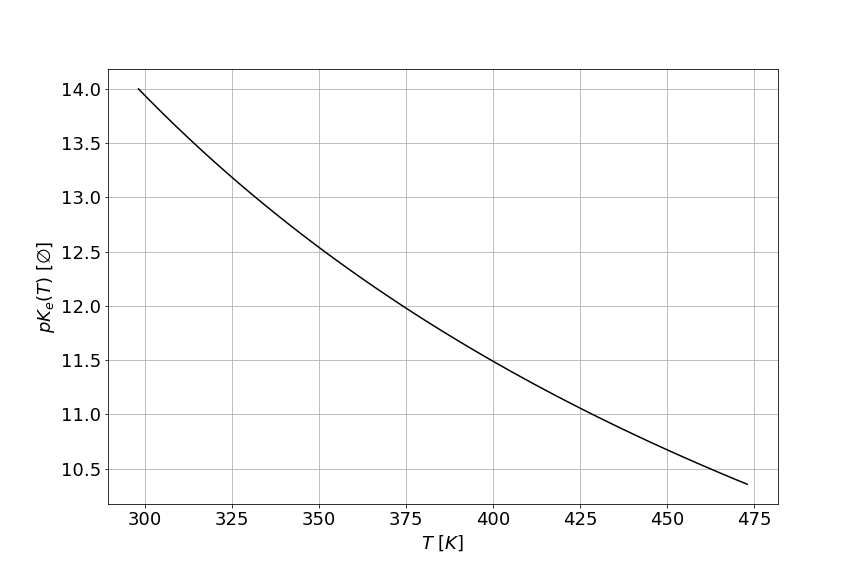
\includegraphics[width=\textwidth]{figures/Corr04}
\end{minipage}\begin{minipage}{0.28\textwidth}
\captionof{figure}{\'{E}volution de la constante d'autoprotolyse, sous forme $pK_e$, avec la température.}
\end{minipage}
\end{center}

\textbf{Relation :} [\textbf{1.0}]

\begin{align*}
K_e(T) = K_e (25 ~ \si{\celsius}) \exp \left[ \frac{\Delta_r H^\circ}{R} \left( \frac{1}{T_{25}} - \frac{1}{T} \right) \right]
\end{align*}

\textbf{AN :} \`{A} $200$, on trouve que : [\textbf{0.5}]
\begin{align*}
pK_e = 10.4
\end{align*}

On sait que l'autoprotolyse de l'eau s'écrit : 
\begin{align*}
\ce{H2O (l) = H^+ (aq) + HO^- (aq)}
\end{align*}

Ceci se traduit par le fait que $[H^+] = [HO^-]$ en présence uniquement d'eau, soit : 

\begin{align*}
[H^+] = [HO^-] = \sqrt{K_e}
\end{align*}

On doit que $pK_e$ a diminué, par conséquent, on a : [\textbf{1.0}]
\begin{align*}
\frac{[H^+](200 ~ \si{\celsius})}{[H^+](25 ~ \si{\celsius})} = \sqrt{\frac{K_e (200 ~ \si{\celsius})}{K_e( 25 ~ \si{\celsius} )}}
\end{align*}

\textbf{AN} [\textbf{0.5}]
\begin{align*}
\frac{[H^+](200 ~ \si{\celsius})}{[H^+](25 ~ \si{\celsius})} = \sqrt{\frac{10^{-10.4}}{10^{-14}}} = 10^{1.8}
\end{align*}


On multiplie par quasiment un facteur $100$ la quantité de protons dans le milieu en utilisant une synthèse micro-onde.

\end{solution}
\end{mybox}

Si on prend en compte que la constante d'autoprotolyse de l'eau peut prendre des valeurs autres que celles à température ambiante, la relation Eq. \ref{eq:h_Tamb} peut être réécrite sous la forme : 

\begin{align}
h = \frac{3.2507 - 0.1566 \cdot pK_e +  0.3131 \cdot pH}{0.80168 - 0.00874 \cdot pK_e +  0.01749 \cdot pH}
\label{eq:k_pH_pKe}
\end{align}

\question[3] Vérifier que l'Eq. \ref{eq:k_pH_pKe} est équivalente à l'Eq. \ref{eq:h_Tamb} pour un système à température ambiante. Tracer cette fonction pour $pK_e = 12$, $13$ et $14$.

\begin{mybox}
\begin{solution}[5cm]
\textbf{Equivalence} \`{A} température ambiante, on a $pK_e = 14$, on a donc : [\textbf{1.0}]
\begin{align*}
3.2507 - 0.1566 \times 14 &= 1.0583 \\
0.80168 - 0.00875 \times 14 &= 0.6792
\end{align*}

Au dernier chiffre significatif près, on retrouve bien la relation Eq. \ref{eq:h_Tamb}.

\textbf{Représentation :} [\textbf{2.0}]

\begin{center}
\begin{minipage}{0.68\textwidth}
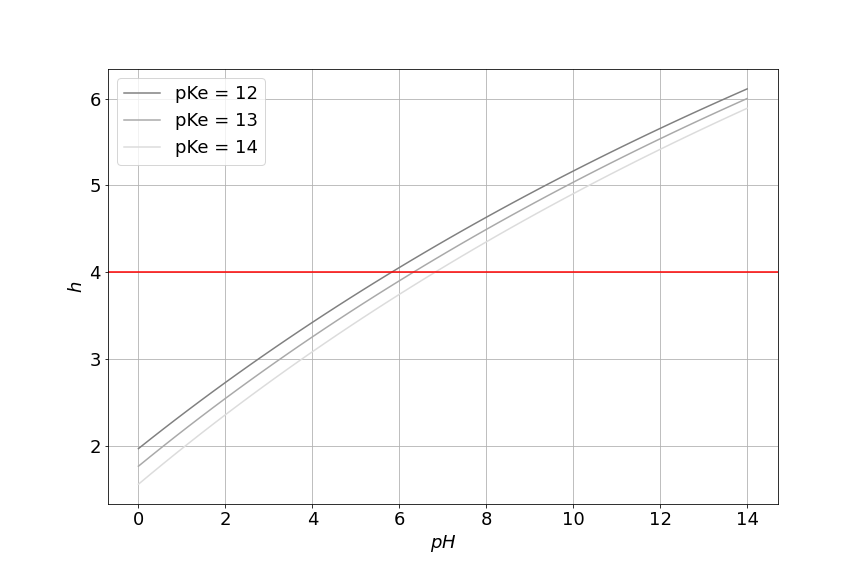
\includegraphics[width=\textwidth]{figures/Corr05}
\end{minipage}\begin{minipage}{0.28\textwidth}
\captionof{figure}{Evolution du taux d'hydrolyse dans de l'eau à différentes températures, c'est-à-dire, à différents $pK_e$}
\end{minipage}
\end{center} 

\end{solution}
\end{mybox}

\question[\half] En déduire l'intérêt des conditions hydrothermales dans cette synthèse.

\begin{mybox}
\begin{solution}[5cm]

On constate qu'une diminution de $pK_e$ a pour conséquence de décaler la courbe vers les $pH$ acides en présence d'un aqua, ce qui se traduit par une acidification du milieu.

\end{solution}
\end{mybox}

Les mécanismes suivants ont été proposés pour la formation de l'anatase, à partir de différents précurseurs : %du précurseur $h=4$ et $h=3$, et du rutile $h=2$ : 

\begin{figure}[H]
\begin{center}
\begin{tabular}{c}
\subfloat[\label{fig:TP1-03a}]{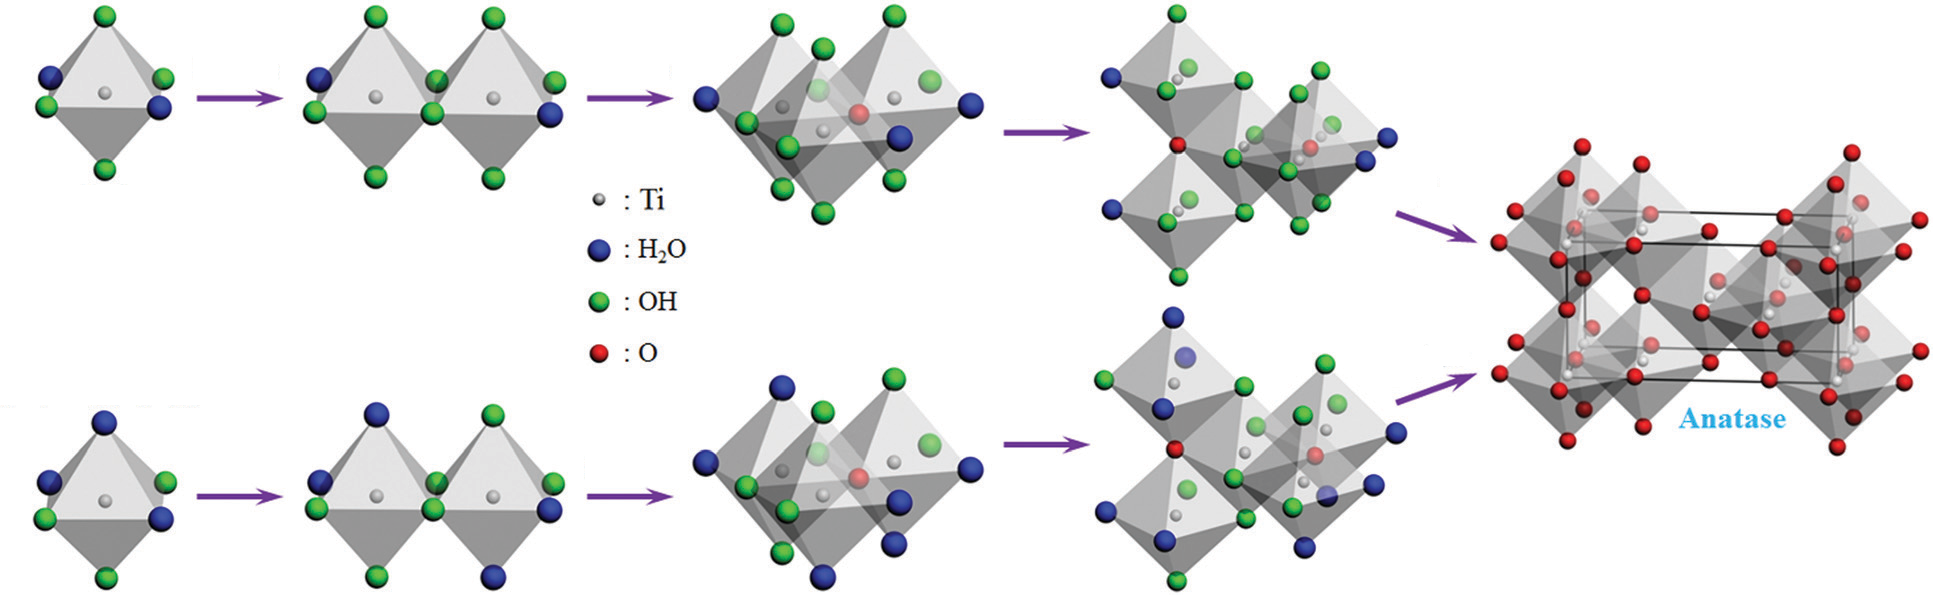
\includegraphics[width=12cm]{figures/Fig03a}} \\ \subfloat[\label{fig:TP1-03b}]{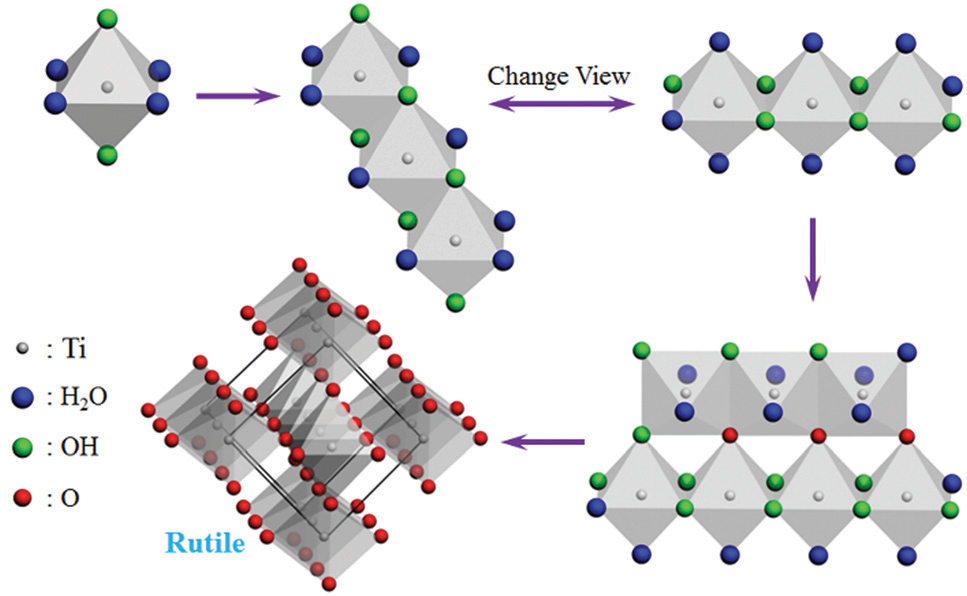
\includegraphics[width=7cm]{figures/Fig03b}}
\end{tabular}
\end{center}
\caption{Mécanisme de formation de l'anatase et du rutile.}
\end{figure}



\question[2] \'{E}crire mécanistiquement une olation et une oxolation.

\begin{mybox}
\begin{solution}[5cm]

\textbf{Oxolation :} Réaction de condensation entre deux complexes coordinés par des ligands hydroxo \ce{HO^-}
\begin{align*}
\ce{2 [ML_n(OH)]^z -> [L_nM-O-ML_n]^{2z} + H2O}
\end{align*}

\textbf{Olation :} Réaction de condensation entre deux complexes coordinés par des ligands aqua \ce{H2O} ou entre ligands aqua et hydroxo.
\begin{align*}
\ce{2 [ML_n(OH2)]^z &-> [L_nM-OH-ML_n]^{2z-1} + H2O + H^+} \\
\text{ou }\ce{[ML_n(OH)]^{z'} + [ML_n(OH2)]^z &-> [L_nM-OH-ML_n]^{z+z'} + H2O}
\end{align*}

\end{solution}
\end{mybox}

\question[2\half] Après avoir identifié le précurseur à l'origine de chacune des voies de synthèse, identifier le type d'acte élémentaire mis en jeu dans ces mécanismes. Justifier que l'on n'observe qu'un seul type d'acte élémentaire ?

\begin{mybox}
\begin{solution}[5cm]

Pour l'anatase, on constate qu'il existe deux voies de synthèse à partir des précurseurs : [\textbf{1.0}]
\begin{align*}
h=4 & \quad \ce{[Ti(OH)4(H2O)2]^0} \\
h=3 & \quad \ce{[Ti(OH)3(H2O)3]^{+}}
\end{align*}

Pour le rutile, on constate qu'il existe un seule voie de synthèse à partir des précurseurs : [\textbf{0.5}]
\begin{align*}
h=2 & \quad \ce{[Ti(OH)2(H2O)4]^{2+}}
\end{align*}

Dans tous ces mécanismes, on part de précurseurs cationiques ou de charge nul, conduisant à la formation en solution d'intermédiaires polycationiques. Pour ce type de composé, on s'attend à avoir plutôt des mécanismes par oxolation, ce qui est effectivement le cas au vu du ligand pontant dans les intermédiaires des différentes voies. [\textbf{1.0}]


\end{solution}
\end{mybox}


\bonusquestion[4] \`{A} partir du modèle des charges partielles, remonter à l'équation \ref{eq:h_Tamb}. 

On rappelle que l'électronégativité moyenne des hydrolysates est donnée par l'équation :

\begin{align*}
\chi = \frac{\sum_i \sqrt{\chi_i^\circ} + 1.36 Z}{\sum_i \frac{1}{\sqrt{\chi_i^\circ}}}
\end{align*}

avec $\chi_i^\circ$ l'électronégativité d'Allred-Rochow de chaque atome neutre.

On précise que l'électronégativité moyenne des hydrolysates est égale à l'électronégativité moyenne d'une solution aqueuse et vaut : 

\begin{align*}
\chi = \chi_{\ce{H2O}} = 2.7321 - 0.0345 \cdot pH
\end{align*}

On rappelle que l'électronégativité dans l'échelle d'Allred-Rochow s'exprime comme : 

\begin{center}
\begin{minipage}{0.48\textwidth}
\begin{tabular}{cccc}
\toprule
\'{E}lèment & \ce{H} & \ce{O} & \ce{Ti} \\
\midrule
Electronegativité moyenne & 2.10 & 3.50 & 1.32 \\
\bottomrule
\end{tabular}
\end{minipage}\begin{minipage}{0.48\textwidth}
\captionof{table}{Electronégativités dans l'échelle d'Allred-Rochow}
\end{minipage}

\end{center}

\begin{mybox}
\begin{solution}[5cm]

On va utiliser le modèle des charges partielles, vu en cours de chimie sol-gel. On décompose le complexe en différents atomes : [\textbf{1.0}]
\begin{align*}
1\ce{Ti} + (6-h+h) \ce{O} + ((6-h) \times 2 + h) \ce{H} = 1 ~ \ce{Ti} + 6 ~ \ce{O} + 12 - h ~ \ce{H}
\end{align*}

La charge totale $Z$ dépend du taux d'hydrolyse $h$ : $Z = 4 - h$.

On en tire donc que : [\textbf{1.0}]

\begin{align*}
\chi = \frac{\sqrt{\chi_{Ti}} + 6\sqrt{\chi_{O}} + (12 - h) \sqrt{\chi_{H}} + 1.36 (4 - h)}{\frac{1}{\sqrt{\chi_{Ti}}} + \frac{6}{\sqrt{\chi_{O}}} + \frac{12-h}{\sqrt{\chi_{H}}}} = 2.7321 - 0.0345 \cdot pH
\end{align*}

En réarangeant l'expression, on trouve une relation du type : [\textbf{2.0}]
\begin{align*}
h = \frac{A + B pH}{C + D pH}
\end{align*}

avec 

\begin{align*}
A &= 2.7321 \cdot \left( \frac{1}{\sqrt{\chi_{Ti}}} + \frac{6}{\sqrt{\chi_{O}}} + \frac{12}{\sqrt{\chi_{H}}}\right) - ( \sqrt{\chi_{Ti}} + \sqrt{\chi_{O}} + \sqrt{\chi_{H}}) - 5.44 \\
B &= 0.0345 \cdot \left( \frac{1}{\sqrt{\chi_{Ti}}} + \frac{6}{\sqrt{\chi_{O}}} + \frac{12}{\sqrt{\chi_{H}}}\right) \\
C &= \frac{2.7321}{\sqrt{\chi_H}} - (1.36 + \sqrt{\chi_H}) \\
D &= - \frac{0.0345}{\sqrt{\chi_H}}
\end{align*}

\end{solution}
\end{mybox}

\setcounter{foo}{\value{question}}

\end{questions}

\newpage

\section*{Barème}

\begin{minipage}{0.33\textwidth}
Noms-Prénoms du binôme
\end{minipage}\begin{minipage}{0.33\textwidth}
$n^\circ 1$ :
\end{minipage}\begin{minipage}{0.33\textwidth}
$n^\circ 2$ :
\end{minipage}

\begin{questions}
\setcounter{question}{\thefoo}

\titledquestion{Cahier de laboratoire}[6] Tenue du cahier de laboratoire.

%\titledquestion{Investissement}[2] Variable d'ajustement à la liberté du correcteur en fonction de l'investissement, de la qualité des raisonnements et de la démarche d'investigation du binôme.

\end{questions}

\begin{center}
\gradetable
\bonusgradetable
\end{center}

\end{document}
